% nuclear_model_combined.tex
% Summary of the MicroBooNE data/MC comparison for the nuclear model
%   LFG26_24a_00_000  =  N/LFG + F_A^LQCD + hA2018
% against the AR23 and MicroBooNE reference tunes.
%
% Figures (in this directory) produced by:
%   run_nuisance_paper_plot.py  ->  Analysis.GENIE().paper_plot(samples, ps, path)
%   ps = [LFG26_24a_00_000, AR23_20i_00_001, G18_10a_02_12a]
%   NUISANCE inputs: /exp/dune/data/users/liangliu/runarea/INCL/nuisance/<tune>.comp.root
%
% Compile (tectonic in the dedicated env):
%   pixi run --manifest-path /exp/dune/data/users/liangliu/texenv/pixi.toml \
%            tectonic --outdir . nuclear_model_combined.tex

\documentclass[11pt]{article}

\usepackage[margin=1in]{geometry}
\usepackage{amsmath}
\usepackage{graphicx}
\usepackage{subcaption}
\usepackage{booktabs}

\graphicspath{{./}}

\newcommand{\dpt}{\delta p_{T}}
\newcommand{\dat}{\delta\alpha_{T}}
\newcommand{\FALQCD}{F_{A}^{\mathrm{LQCD}}}

\title{Nuclear-model comparison against MicroBooNE charged-current data:\\
       N/LFG $+\ \FALQCD\ +$ hA2018}
\author{}
\date{}

\begin{document}
\maketitle

\section*{Summary}

Figure~\ref{fig:nuclear_model_combined} compares the GENIE prediction built from
a nucleon-level local Fermi gas (N/LFG) nuclear ground state, a lattice-QCD axial
form factor ($\FALQCD$), and the hA2018 final-state-interaction (FSI) cascade
---sample \texttt{LFG26\_24a\_00\_000} (solid)--- against the MicroBooNE
charged-current cross-section data (points) and two empirical reference tunes,
AR23 and the MicroBooNE tune (drawn dashed in the projected panels). The samples
are summarised in Table~\ref{tab:samples}.

Panels (a)--(d) use the CC\,$1\mu1p$ transverse-kinematic-imbalance (TKI) sample:
the single-transverse momentum imbalance $\dpt$ and boosting angle $\dat$, with
the two-dimensional $\dpt$ shown in the most back-to-back ($\dat<45^{\circ}$) and
most FSI-disturbed ($135^{\circ}<\dat<180^{\circ}$) angular slices. Panels
(e)--(f) use the CC\,$1\mu Np$ sample: the muon momentum $p_{\mu}$ and the
leading-proton momentum $p_{p}$. The TKI observables isolate nuclear effects:
$\dpt$ is driven by Fermi motion and FSI, while the migration of strength toward
$\dat\!\to\!180^{\circ}$ reflects the FSI-induced momentum loss of the outgoing
proton.

Replacing the empirical references with the explicit N/LFG ground state, lattice
$\FALQCD$, and hA2018 cascade, \texttt{LFG26\_24a\_00\_000} reproduces the bulk of
the $\dpt$ distribution and the $p_{\mu}$/$p_{p}$ spectra. At the $\dpt$ peak it
sits highest of the three predictions and closest to the data, whereas AR23
underpredicts the peak; the predictions converge in the high-$\dpt$ tail where
single-nucleon kinematics no longer dominate.

\begin{table}[h]
\centering
\begin{tabular}{lll}
\toprule
GENIE sample & Nuclear model & Role \\
\midrule
\texttt{LFG26\_24a\_00\_000} & N/LFG $+\ \FALQCD\ +$ hA2018 & this work (solid) \\
\texttt{AR23\_20i\_00\_001}  & AR23 tune                    & reference (dashed) \\
\texttt{G18\_10a\_02\_12a}   & MicroBooNE tune              & reference (dashed) \\
\bottomrule
\end{tabular}
\caption{The three GENIE samples overlaid on the MicroBooNE data. The $a$/$b$
suffix in the \texttt{LFG26} naming selects the FSI model (here \texttt{a}\,=\,
hA2018); the leading digits select the ground state (LFG) and the axial form
factor ($\FALQCD$).}
\label{tab:samples}
\end{table}

\begin{figure}[p]
  \centering
  \begin{subfigure}[t]{0.49\textwidth}
    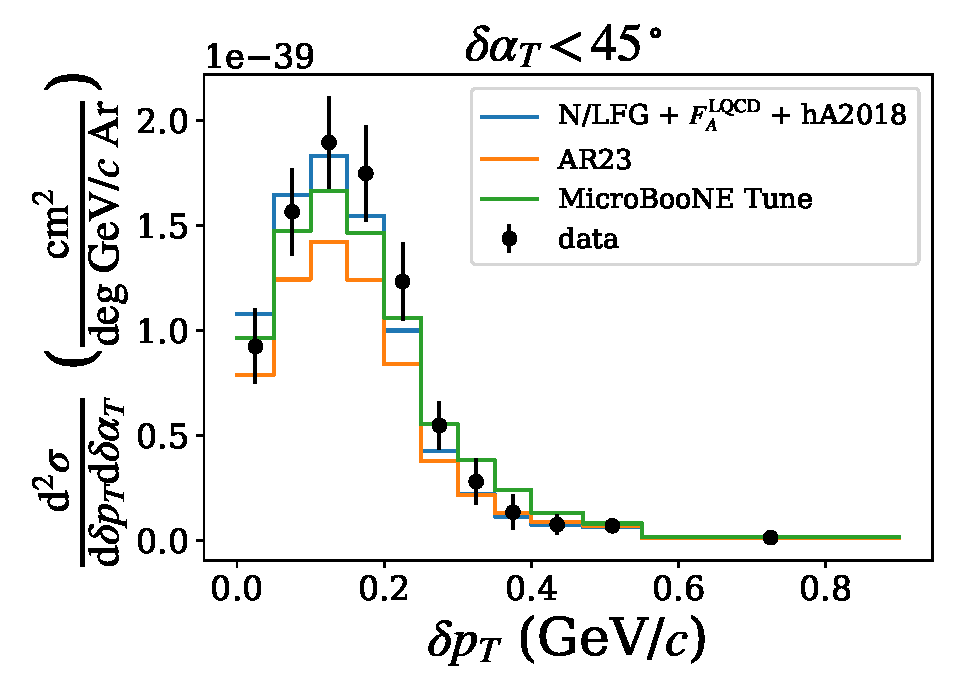
\includegraphics[width=\linewidth]{nuisance_lfg26_24a_ar23_ub_a.pdf}
    \caption{$\dpt$ ($\dat<45^{\circ}$)}
  \end{subfigure}\hfill
  \begin{subfigure}[t]{0.49\textwidth}
    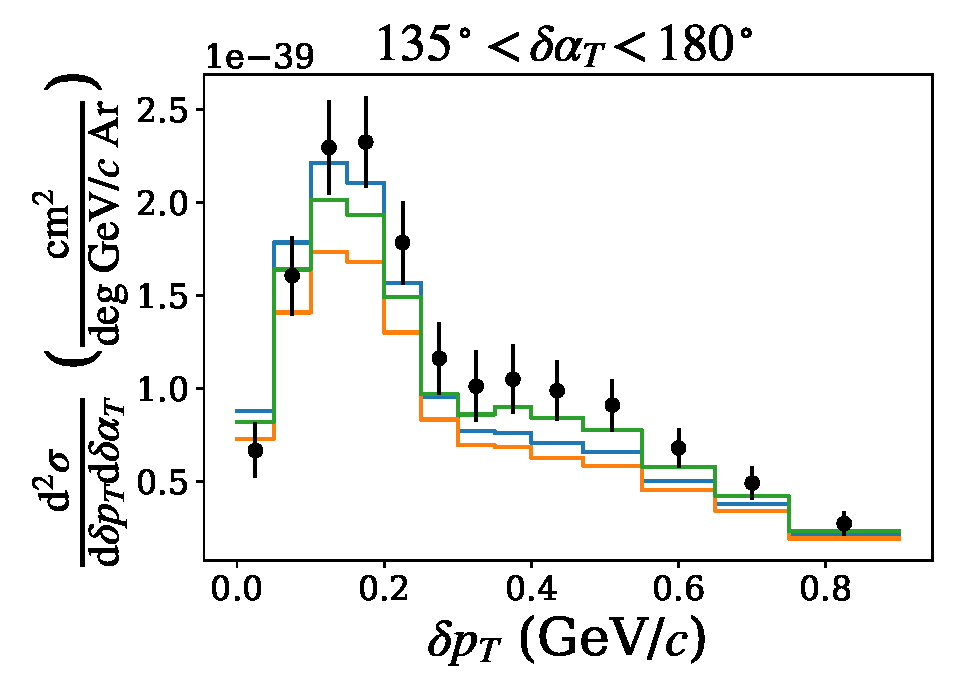
\includegraphics[width=\linewidth]{nuisance_lfg26_24a_ar23_ub_b.pdf}
    \caption{$\dpt$ ($135^{\circ}<\dat<180^{\circ}$)}
  \end{subfigure}

  \medskip
  \begin{subfigure}[t]{0.49\textwidth}
    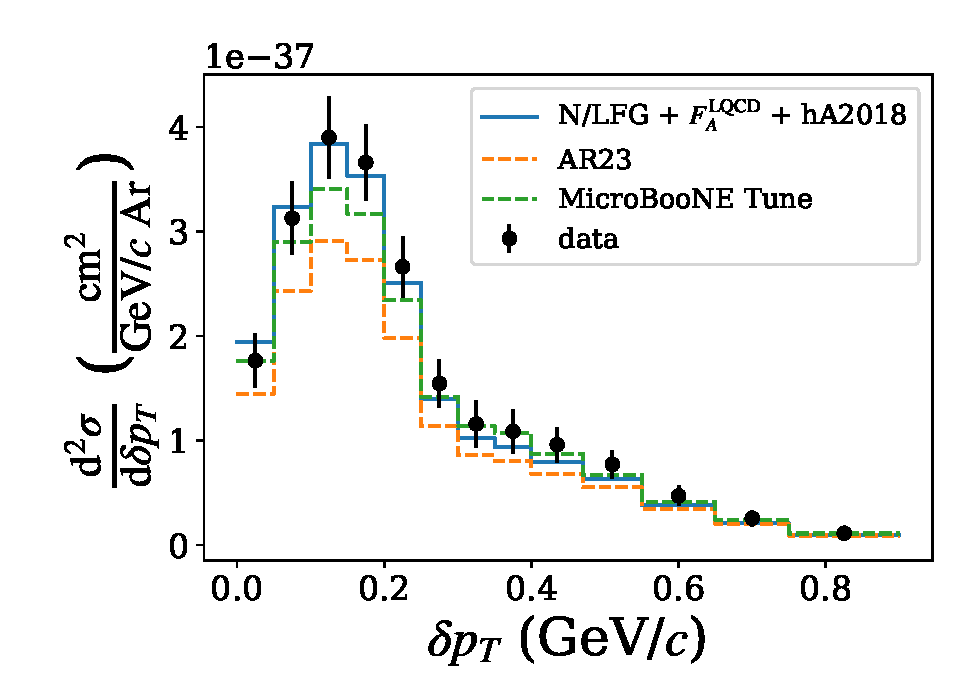
\includegraphics[width=\linewidth]{nuisance_lfg26_24a_ar23_ub_c.pdf}
    \caption{$\dpt$}
  \end{subfigure}\hfill
  \begin{subfigure}[t]{0.49\textwidth}
    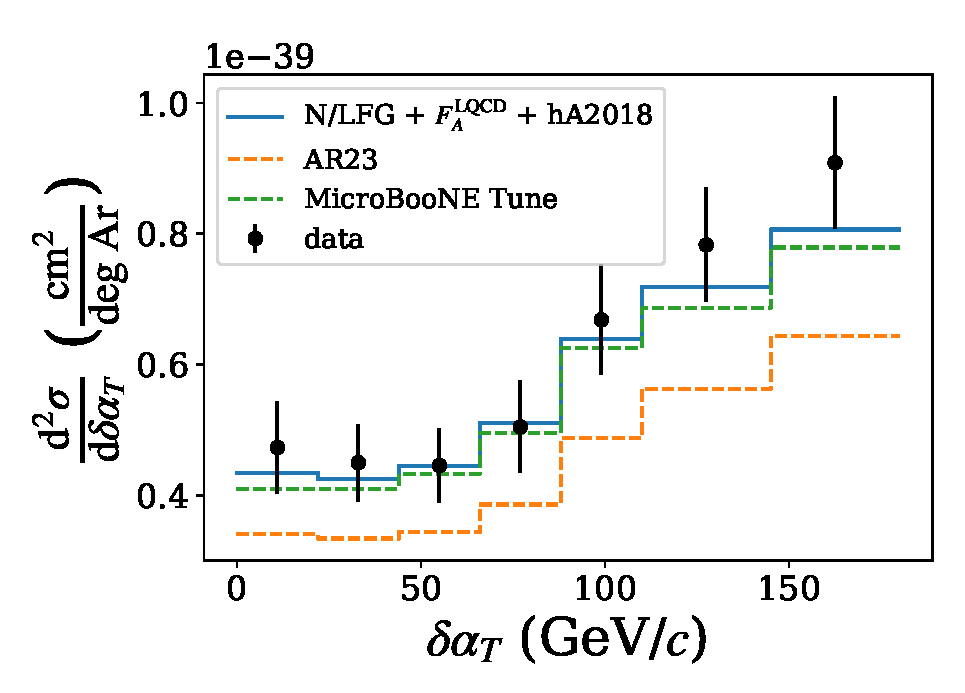
\includegraphics[width=\linewidth]{nuisance_lfg26_24a_ar23_ub_d.pdf}
    \caption{$\dat$}
  \end{subfigure}

  \medskip
  \begin{subfigure}[t]{0.49\textwidth}
    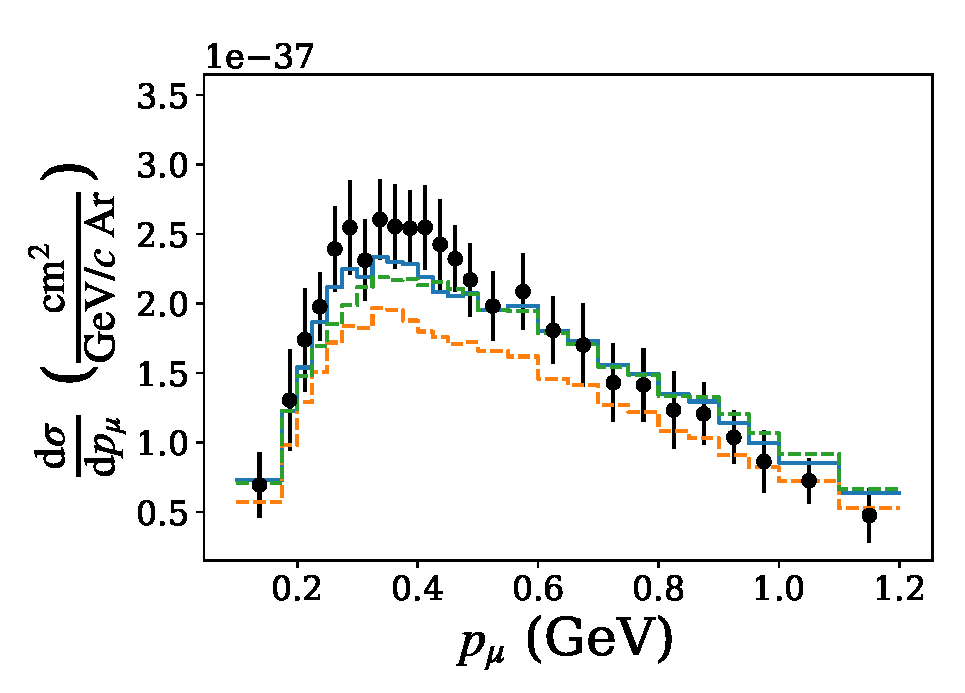
\includegraphics[width=\linewidth]{nuisance_lfg26_24a_ar23_ub_e.pdf}
    \caption{$p_{\mu}$}
  \end{subfigure}\hfill
  \begin{subfigure}[t]{0.49\textwidth}
    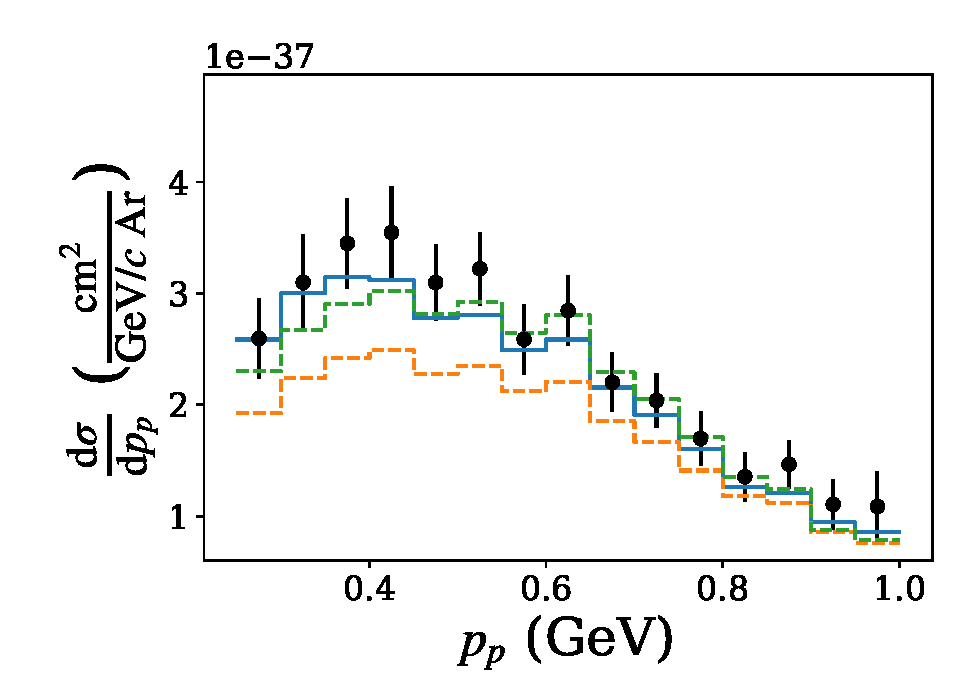
\includegraphics[width=\linewidth]{nuisance_lfg26_24a_ar23_ub_f.pdf}
    \caption{$p_{p}$}
  \end{subfigure}

  \caption{MicroBooNE charged-current cross sections (black points) compared with
  the N/LFG $+\ \FALQCD\ +$ hA2018 model \texttt{LFG26\_24a\_00\_000} (solid blue)
  and the AR23 and MicroBooNE reference tunes (dashed in panels (c)--(f)).
  (a)--(b) two-dimensional
  $\dpt$ in the lowest and highest $\dat$ slices of the CC\,$1\mu1p$ TKI
  measurement; (c)--(d) the projected $\dpt$ and $\dat$; (e)--(f) the muon and
  leading-proton momenta from the CC\,$1\mu Np$ measurement.}
  \label{fig:nuclear_model_combined}
\end{figure}

\end{document}
